\input{sep3-annotated-ott}
\input{sep3-unannotated-ott}

\renewcommand{\Sepdrulename}[1]{\scriptsize \textsc{#1}}
\renewcommand{\SepUdrulename}[1]{\scriptsize \textsc{#1}}
% See the seppp.tex file for reminders of the motivation of the
% design.

The previous chapter introduced the freedom of speech
dependently-typed functional programming language. This language
contained two fragments, the logical fragment and the programmatic
fragment.  However, these fragments are judgmentally kept separate.
That is the syntax was the same for both fragments, even more so the
syntax for programs and types are collapsed into a single syntactic
category.  Thus, the fragments are not strictly separate, but rather,
weakly so.  This particular design is very appealing because it has an
elegant definition, but this elegance comes at a cost.  The type
system suffers from many value restrictions, and as we have said
above, this makes programming very hard.

Consider a design where instead of a weak separation of the two
fragments -- logical and programmatic -- we insist on a strict one.
That is the logical fragment and the programmatic fragment have
completely distinct languages for types and programs, and then the two
fragments are related using freedom of speech by typing rules.  So we
go from a picture that looks like this:
\begin{center}
  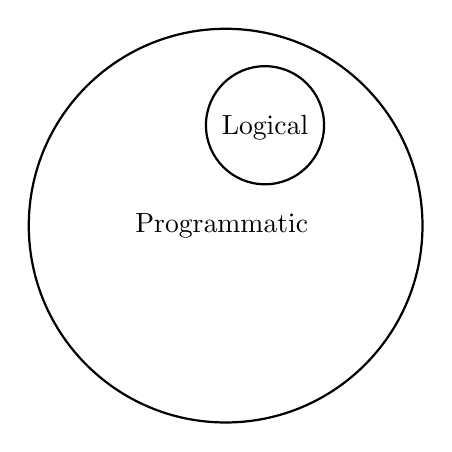
\begin{tikzpicture}[scale=2.5,cap=round,>=latex]    
    \draw[thick] (2.8cm,0cm) circle(1cm);
    \draw (2.78cm,0cm) node {Programmatic};
    \draw[thick] (3cm,0.51cm) circle(0.3cm);
    \draw (3cm,0.5cm) node {Logical};
  \end{tikzpicture}
\end{center}
To the following picture:
\begin{center}
  \begin{tikzpicture}[>=stealth',shorten >=1pt,auto,node distance=5 cm, scale = 1, transform shape]
    \node[state, minimum size=83.1pt] (A)              {Logical};
    \node[state] (B) [right of=A] {Programmatic};

    \path[->] (A) edge [bend left] (B)
              (B) edge [bend left] (A);
  \end{tikzpicture}    
\end{center}
We have seen this diagram before in the previous chapter, but there it
was used to give an intuitive understanding of the free speech
property, but the two fragments are not strictly separate.  Now we
insist that they are in fact strictly separate, and the first diagram
above is no long applicable unlike the freedom of speech language.  We
will see that this separation allows for the lifting of all value
restrictions from the typing rules.  

The freedom of speech language is not a very expressive programming
language.  For example, we did not show how to construct full
programs, nor did freedom of speech contain any notion of abstract
data types or pattern matching.  Thus, it is rather difficult to
consider freedom of speech as a real-world programming language.  In
this chapter we introduce the design of a new programming language
called Separation of Proof from Program ($\Sep$) that contains all of
these new features.  The logical and programmatic fragments are
strictly separate, and $\Sep$ is a full real-world programming
language complete with abstract datatypes and pattern matching.  There
are also additional features that we will introduce below.  The
definition of $\Sep$ is very large with over a hundred typing rules
and a large amount of syntax.  Therefore, we do not have the space to
introduce the complete definition in the same style as we did for
freedom of speech, but instead concentrate on the most important
aspects of the design.  If the reader wishes to wade through the
entire definition please see
Appendix~\ref{sec:annotated_separation_of_proof_from_program} and
Appendix~\ref{sec:unannotated_separation_of_proof_from_program}, but
the reader may wish to read this chapter first to understand the need
for two appendices.

\begin{center}
  \small
  \begin{math}
    \begin{array}{llllllllllllllll}
      \text{(Programs) }    [[prog]] ::= [[pdef]] \mid [[prog pdef]]\\
      \\
      \text{(Definitions) } [[pdef]] ::= [[datatype_decl]] \mid [[predicateType x :: LK]] \mid
      [[predef x = P]] \mid \\
      [[theorem x :: P]] \mid [[prfdef x = p]] \mid [[type x :: t]] \mid [[termdef x = t]] \\
      \\
      \text{(Datatype Types) } [[dt]] ::= [[Pi x : A . dt]] \mid [[Type i]]\\
      \\
      \text{(Datatypes) }   [[datatype_decl]] ::= [[data Ctor C t where M]]\\
      \\
      \text{(Stages) }      [[ep]]   ::= [[+]] \mid [[-]]\\
      \\
      \text{(Classifiers) } [[ks]]   ::= [[L]] \mid [[P]]\\
      \\
      \text{(Argument Classifiers) } Arg, A ::= [[term]] \mid [[predicate]] \mid LK\\
      \\
      \text{(Logical Argument Classifiers) } [[W]] ::= [[Type]] \mid [[Formula i]]\\
      \\
      \text{(Super Kinds) } [[L]] ::= [[Logical i]]\\
      \\
      \text{(Base Kinds) }  [[Ti]] ::= [[Type i]] \mid [[Formula i]]\\
      \\
      \text{(Logical Kind) } [[LK]] ::= [[x]] \mid [[Formula i]] \mid [[Forall x : A.LK]]\\
      \\
      \text{(Arguments) } [[a]] ::= [[term]] \mid [[proof]] \mid [[predicate]]\\
      \\
      \text{(Predicates) } [[predicate]], [[P]] ::= [[x]] \mid [[\ L x : A . P]] \mid [[P a]] \mid [[Forall x : A . P]] \mid [[let x = p in P]] \mid [[let x = P in P']] \mid \\
      [[let x = t [ p ] in P]] \mid [[t1 = t2]] \mid [[t !]] \mid [[P1 + P2]] \mid [[Exists x : A . P]] \mid [[bot i]] \mid [[t < t']] \\
      \\
      \text{(Proofs) } [[proof]],[[p]] ::= [[x]] \mid [[injl p with P]] \mid [[injr p with P]] \mid [[case p of x . p' , y . p'']] \mid [[\ L x : A . p]] \mid [[p a]] \mid \\
      [[(a , p ) as P]] \mid [[case p1 of ( x , y ) . p2]] \mid [[let x = p' in p]] \mid [[let x = P in p]] \mid [[let x = t [ y ] in p]] \mid [[join t1 t2]] \mid \\ 
      [[conv p by q1 ... qn at x1 ... xm . P]] \mid [[predconv p P]] \mid [[valax t]] \mid [[ord t t']] \mid [[case t [ x ] p of R]] \mid\\
      [[tcase t [ x ] of abort -> p1 | ! -> p2]] \mid [[ind f x : t , p1 . p2]] \mid [[contra p1]] \mid [[contraval p1 p2]]\\
      \\
      \text{(Proof Values) } [[pv]] ::= [[\ L x : A . p]] \mid [[conv pv by q1 ... qn at x1 ... xm . P]] \mid [[valax t]]\\
      \\
      \text{(Terms) } [[term]],[[t]],[[w]] ::= [[x]] \mid [[Type i]] \mid [[Pi ep x : A . t]] \mid [[\ P ep x : A . t]] \mid [[let x = p in t]] \mid [[let x = P in t]] \mid \\
      [[let x = t [ y ] in t']] \mid [[conv t by q1 ... qn at x1 ... xm . t']] \mid [[case t [ x ] of H]] \mid [[tcast t by p]] \mid [[t a ep]] \mid \\
      [[abort t]] \mid [[rec f x : t1 . t2]] \mid [[Ctor C]]\\      
    \end{array}
  \end{math}
\end{center}
\begin{center}
  \begin{math}
    \begin{array}{llllllllllllllllll}
      \text{(Term Values) } [[tv]] ::= [[Type i]] \mid [[Pi ep x : A . t]] \mid [[\ P ep x : A . t]] \mid [[rec f x : t1 . t2]] \mid [[Ctor C tv1 ep1 dots tvn epn]]\\
      \\
      \text{(Expressions) } [[exp]],[[e]] ::= [[L]] \mid [[LK]] \mid [[predicate]] \mid [[proof]] \mid [[term]]\\
      \\
      \text{(Conversions) } [[q]] ::= [[proof]] \mid [[t1 = t2]]\\
      \\
      \text{(Proof Branches) } [[R]] ::= [[Ctor C x1 ep1 dots xn epn => p | R]] \mid [[done]]\\
      \\
      \text{(Term Branches) } [[H]] ::= [[Ctor C x1 ep1 dots xn epn => t | H]] \mid [[done]]\\
      \\
      \text{(Value Annotations) } [[g]] ::= [[val]]\\
      \\
      \text{(Typing Contexts) } [[G]] ::= [[.]] \mid [[G , x : g e]] \mid [[G , x : e]] \mid [[G1 , G2]]\\
      \\
      \text{(Typing Signature) } [[D]] ::= [[.]] \mid [[D , ( C , t , M )]] \mid [[D , x = ( a , A )]] \mid [[D1 , D2]]\\
      \\
      \text{(Term Lists) } [[tl]] ::= [[nil]] \mid [[t :: tl]] \mid [[_]]\\
      \\
      \text{(Constructor Sets) } [[l]] ::= [[empty]] \mid [[{ Ctor C : t'}]] \mid [[l1 inter l2]] \mid [[l1 - l2]] \mid [[l1 = l2]]\\
      \\
      \text{(Constructor Lists) } [[M]] ::= [[nil]] \mid [[Ctor C : t']] \mid [[M1 :: M2]]\\
      \\
      \text{(Indicies) } [[i]] ::= 1 \mid 2 \mid 3 \mid \cdots\\        
    \end{array}
  \end{math}
\end{center}

\begin{figure}
  \begin{mathpar}
    \SepdrulePBEqXXApp{} \and
    \SepdrulePBEqXXLetOne{} \and
    \SepdrulePBEqXXLetTwo{} \and
    \SepdrulePBEqXXLetThree{}
  \end{mathpar}
  \caption{Predicate $\beta$-Equality}
  \label{fig:pred-beta-eq}
\end{figure}

\begin{figure}
  \begin{mathpar}
    \SepdruleSigXXOkXXEmpty{} \and
    \SepdruleSigXXOkXXExtData{} \and
    \SepdruleSigXXOkXXExtGDef{}
  \end{mathpar}
  \caption{Well-defined Typing Signatures}
  \label{fig:sig-ok}
\end{figure}

\begin{figure}
  \begin{mathpar}
    \SepdruleCtxXXOkXXEmpty{} \and
    \SepdruleCtxXXOkXXExtTerm{} \and
    \SepdruleCtxXXOkXXExtLK{} \and
    \SepdruleCtxXXOkXXExtPred{}
  \end{mathpar}
  \caption{Well-defined Tying Contexts}
  \label{fig:ctx-ok}
\end{figure}

\begin{figure}
  \begin{mathpar}
    \SepdruleTYPGXXDataTypeDeclaration{}  \and
    \SepdruleTYPGXXPredicateType{} \and
    \SepdruleTYPGXXPredicate{} \and
    \SepdruleTYPGXXTheorem{} \and
    \SepdruleTYPGXXProof{} \and
    \SepdruleTYPGXXType{} \and
    \SepdruleTYPGXXTerm{} \and
    \SepdruleTYPGXXStep{}
  \end{mathpar}
  \caption{Program Type-checking Rules}
  \label{fig:prog-ty}
\end{figure}

\begin{figure}
  \begin{mathpar}
    \SepdrulePVXXProof{} \and
    \SepdrulePVXXTerm{}
  \end{mathpar}
  \caption{Values or Proofs}
  \label{fig:vorp}
\end{figure}

\begin{figure}
  \begin{mathpar}
    \SepdruleVXXVar{} \and
    \SepdruleVXXType{} \and
    \SepdruleVXXPi{} \and
    \SepdruleVXXLamPlus{} \and
    \SepdruleVXXLamMinus{} \and
    \SepdruleVXXRec{} \and
    \SepdruleVXXCtor{} \and
    \SepdruleVXXtCast{}
  \end{mathpar}
  \caption{Semantic Values}
  \label{fig:sem-val}
\end{figure}

\begin{figure}
  \begin{mathpar}
    \SepdruleDdXXEmpty{} \and
    \SepdruleDdXXBranch{}
  \end{mathpar}
  \caption{Constructor List Type-checking Rules}
  \label{fig:cons-list-ty}
\end{figure}

\begin{figure}
  \begin{mathpar}
    \SepdruleDataDecl{}
  \end{mathpar}
  \caption{Datatype Type-checking Rules}
  \label{fig:datatype-ty}
\end{figure}

\begin{figure}
  \begin{mathpar}
    \SepdrulePBXXDone{} \and
    \SepdrulePBXXBranch{}
  \end{mathpar}
  \caption{Proof branches Type-checking Rules}
  \label{fig:PB-ty}
\end{figure}

\begin{figure}
  \begin{mathpar}
    \SepdruleTBXXDone{} \and
    \SepdruleTBXXBranch{}
  \end{mathpar}
  \caption{Term branches Type-checking Rules}
  \label{fig:TB-ty}
\end{figure}

\begin{figure}
  \begin{mathpar}
    \SepdruleEqProof{} \and
    \SepdruleEqGen{}
  \end{mathpar}
  \caption{Type-checking Rules for Conversions}
  \label{fig:ty-convs}
\end{figure}

\begin{figure}
  \begin{mathpar}
    \SepdruleGlobalDef{}
  \end{mathpar}
  \caption{Type-checking Rules for Global Definitions}
  \label{fig:ty-global-def}
\end{figure}

\begin{figure}
  \begin{mathpar}
    \SepdruleLKXXFormula{} \and
    \SepdruleLKXXPredicate{}
  \end{mathpar}
  \caption{Type-checking Rules for Logical Kinds}
  \label{fig:logical-ty}
\end{figure}

\begin{figure}
  \scriptsize
  \begin{mathpar}
    \SepdrulePRDXXVar{} \and
    \SepdrulePRDXXGD{} \and
    \SepdrulePRDXXBtm{} \and
    \SepdrulePRDXXDisj{} \and
    \SepdrulePRDXXForallOne{} \and
    \SepdrulePRDXXForallTwo{} \and
    \SepdrulePRDXXForallThree{} \and
    \SepdrulePRDXXForallFour{} \and
    \SepdrulePRDXXExtOne{} \and
    \SepdrulePRDXXExtTwo{} \and
    \SepdrulePRDXXExtThree{} \and
    \SepdrulePRDXXExtFour{} \and
    \SepdrulePRDXXLetPF{} \and
    \SepdrulePRDXXLetPRD{} \and
    \SepdrulePRDXXLet{} \and
    \SepdrulePRDXXKXXEq{} \and
    \SepdrulePRDXXTRM{} \and
    \SepdrulePRDXXLam{} \and
    \SepdrulePRDXXApp{}
  \end{mathpar}
  \caption{Type-checking Rules for Predicates}
  \label{fig:pred-ty}
\end{figure}

\begin{figure}
  \scriptsize
  \begin{mathpar}
    \SepdrulePRFXXVar{} \and
    \SepdrulePRFXXGD{}  \and
    \SepdrulePRFXXExti{}  \and
    \SepdrulePRFXXExtE{}  \and
    \SepdrulePRFXXInl{} \and
    \SepdrulePRFXXInr{} \and
    \SepdrulePRFXXOrElim{} \and
    \SepdrulePRFXXFT{} \and
    \SepdrulePRFXXFPRD{} \and
    \SepdrulePRFXXFLK{} \and
    \SepdrulePRFXXApp{} \and
    \SepdrulePRFXXLetPRF{} \and
    \SepdrulePRFXXLetPRD{} \and
    \SepdrulePRFXXLet{} \and
    \SepdrulePRFXXJoin{} \and
    \SepdrulePRFXXConv{} \and
    \SepdrulePRFXXPRDConv{} \and
    \SepdrulePRFXXVal{} \and
    \SepdrulePRFXXOrd{} \and
    \SepdrulePRFXXInd{} \and
    \SepdrulePRFXXCTROne{} \and
    \SepdrulePRFXXCTRTwo{} \and
    \SepdrulePRFXXCTRV{} \and
    \SepdrulePRFXXCase{} \and
    \SepdrulePRFXXTCase{} 
  \end{mathpar}
  \caption{Type-checking Rules for Proofs}
  \label{fig:proofs-ty}
\end{figure}

\begin{figure}
  \scriptsize
  \begin{mathpar}
    \SepdruleTRMXXTYZero{} \and
    \SepdruleTRMXXTYi{} \and
    \SepdruleTRMXXPi{} \and
    \SepdruleTRMXXPiPRD{} \and
    \SepdruleTRMXXPiLK{} \and
    \SepdruleTRMXXVar{} \and
    \SepdruleTRMXXtCast{} \and
    \SepdruleTRMXXGD{} \and
    \SepdruleTRMXXDC{} \and
    \SepdruleTRMXXLamPL{} \and
    \SepdruleTRMXXLamMI{} \and
    \SepdruleTRMXXApp{} \and
    \SepdruleTRMXXLetPRF{} \and
    \SepdruleTRMXXLetPRD{} \and
    \SepdruleTRMXXLet{} \and
    \SepdruleTRMXXConv{} \and
    \SepdruleTRMXXRec{} \and
    \SepdruleTRMXXAbort{} \and
    \SepdruleTRMXXCase{}
  \end{mathpar} 
  \caption{Type-checking Rules for Terms}
  \label{fig:ty-terms}
\end{figure}

\begin{figure}
  \scriptsize
  \begin{mathpar}
    \SepUdruleLcbvXXCtxStep{} \and
    \SepUdruleLcbvXXGlobalDef{} \and
    \SepUdruleLcbvXXBetaTerm{} \and
    \SepUdruleLcbvXXBetaProof{} \and
    \SepUdruleLcbvXXBetaSumLeft{} \and
    \SepUdruleLcbvXXBetaSumRight{} \and
    \SepUdruleLcbvXXBetaExt{} \and
    \SepUdruleLcbvXXCaseTerm{} \and
    \SepUdruleLcbvXXTCaseAbort{} \and
    \SepUdruleLcbvXXTCaseVal{} \and
    \SepUdruleLcbvXXInd{} \and
    \SepUdruleLcbvXXLetOne{} \and
    \SepUdruleLcbvXXLetTwo{} \and
    \SepUdruleLcbvXXLetThree{}
  \end{mathpar}
  \caption{CBV Reduction Rules for Unannotated Proofs}
  \label{fig:cbv-red-unprf}
\end{figure}

\begin{figure}
  \scriptsize
  \begin{mathpar}
    \SepUdruleCBVXXCtxStep{} \and
    \SepUdruleCBVXXGlobalDef{} \and
    \SepUdruleCBVXXCtxAbort{} \and
    \SepUdruleCBVXXBeta{} \and
    \SepUdruleCBVXXLet{} \and
    \SepUdruleCBVXXRec{} \and
    \SepUdruleCBVXXTCast{} \and
    \SepUdruleCBVXXCaseTerm{}
  \end{mathpar}
  \caption{CBV Reduction Rules for Unannotated Terms}
  \label{fig:cbv-red-unterm}
\end{figure}


We first define some convenient notation. If $([[Ctor C]], [[t]],
[[M]]) \in [[D]]$ then $[[D]]_1([[Ctor C]]) = [[Ctor C]]$,
$[[D]]_2([[Ctor C]]) = [[t]]$, and $[[D]]_3([[Ctor C]]) = [[M]]$.

{\bf Judgement Descriptions}
\begin{center}
  \begin{tabular}{lll}
    $[[D , G |- M t tl : Ctor C x1 ep1 dots xn epn]]$\\
    &
    \begin{tabular}{lll}
      $[[M]]$  & List of datatype constructors.\\
      $[[t]]$  & Type of datatype being declared.\\
      $[[tl]]$ & Datatype constructor accumulator.\\
      $[[Ctor C x1 ep1 dots xn epn]]$ & The datatype being declared.\\
    \end{tabular}
    & \\
    $[[D , G |-PB R t1 t2 p l : P]]$\\
    &
    \begin{tabular}{lll}
      $[[R]]$  & List of case branches.\\
      $[[t1]]$ & The scrutiny of the case expression.\\
      $[[t2]]$ & The type of the scrutiny.\\
      $[[p]]$  & The proof that the scrutiny equals the pattern.\\
      $[[l]]$  & An accumulator.\\
      $[[P]]$  & The type of the case expression.\\
    \end{tabular}
    & \\
    $[[D , G |-TB H t1 t2 p l : t']]$\\
    &
    \begin{tabular}{lll}
      $[[H]]$  & List of case branches.\\
      $[[t1]]$ & The scrutiny of the case expression.\\
      $[[t2]]$ & The type of the scrutiny.\\
      $[[p]]$  & The proof that the scrutiny has a value.\\
      $[[l]]$  & An accumulator.\\
      $[[t']]$ & The type of the case expression.\\
    \end{tabular}
    & \\
    $[[D , G |- eqpf q ep : P]]$\\
    &
    \begin{tabular}{lll}
      $[[q]]$  & Either a proof of an equality or a trivial axiom of equality.\\
      $[[ep]]$ & The stage of $[[q]]$; $+$ if $[[q]]$ is a proof and $-$ otherwise.\\
    \end{tabular}
  \end{tabular}
\end{center}

\begin{definition}
  \label{def:asep3_togglepol}  
  \begin{center}
    \begin{math}
      \mathsf{togglePol} ([[t]], [[vl]]) = \left\{
        \begin{array}{ll}
          [[Pi - x : y.togglePol(t',vl)]]    & : [[t equiv Pi + x : y.t']] \land \exists [[A]].([[y]]:[[A]]) \in [[vl]]\\
          [[Pi ep x : A . togglePol(t',vl)]] & : \text{otherwise}
        \end{array}
      \right.
    \end{math}
  \end{center}
\end{definition}

\begin{definition}
  \label{def:eraser_function}
  The erasers are defined as follows:
  \begin{itemize}
  \item Super Kinds:\\
    \begin{math}
      \begin{array}{lll}
        |\mathsf{LogicalKind}_{[[i]]}| & = & \mathsf{LogicalKind}_{[[i]]}
      \end{array}
    \end{math}
  \item Logical Kinds:\\
    \begin{math}
      \begin{array}{lll}
        |[[x]]|                   & = & x\\
        |\mathsf{Formula}_{[[i]]}| & = & \mathsf{Formula}_{{[[i]]}}\\
        |[[Forall x : A . LK]]|   & = & \forall [[x]] : |[[A]]|.|[[LK]]|
      \end{array}
    \end{math}
    
  \item Predicates:\\
    \begin{math}
      \begin{array}{lll}
        |[[\ L x : A . P]]|       & = & \Lambda [[x]] . |[[P]]|\\
        |[[P a]]|                 & = & |P|\ |a|\\
        |[[Forall x : A . P]]|    & = & \forall [[x]]:|[[A]]|.|[[P]]|\\
        |[[t1 = t2]]|             & = & |[[t1]]| = |[[t2]]|\\
        |[[t !]]|                 & = & |[[t]]|!\\
        |[[let x = p in P]]|      & = & \mathsf{let}\,[[x]] = |[[p]]|\,in\,|[[P]]|\\
        |[[let x = P in P']]|     & = & \mathsf{let}\,[[x]] = |[[P]]|\,in\,|[[P']]|\\
        |[[let x = t [x'] in P]]| & = & \mathsf{let}\,[[x]] = |[[t]]|\,in\,|[[P]]|\\
        |[[P1 + P2]]|             & = & |[[P1]]| + |[[P2]]|\\
        |[[Exists x : A . P]]|    & = & \exists [[x]]:|[[A]]|.|[[P]]|\\
        |[[bot i]]|               & = & [[bot i]]\\
        |[[t < t']]|              & = & |[[t]]| < |[[t']]|
      \end{array}
    \end{math}
    
  \item Proofs:\\
    \begin{math}
      \begin{array}{lll}
        |[[x]]| & = & x\\
        |[[\ L x : A . p]]| & = & \Lambda [[x]].|[[p]]|\\
        |[[p p']]| & = & |[[p]]|\,|[[p']]|\\
        |[[p t]]| & = & |[[p]]|\,|[[t]]|\\
        |[[injl p with P]]| & = & \mathsf{injl}\,|[[p]]|\\
        |[[injr p with P]]| & = & \mathsf{injr}\,|[[p]]|\\
        |[[case p of x . p' , y . p'']]| & = & \mathsf{case}\,|[[p]]|\,\mathsf{of}\,[[x]] . |[[p']]| , [[y]] . |[[p'']]|\\
        |[[(a , p ) as P]]| & = & (|[[a]]|,|[[p]]|)\\
        |[[case p1 of ( x , y ) . p2]]| & = & \mathsf{case}\,|[[p1]]|\,\mathsf{of}\,( [[x]] , [[y]] ) . |[[p2]]|\\
        |[[let x = p' in p]]| & = & \mathsf{let}\,[[x]] = |[[p']]|\,in\,|[[p]]|\\
        |[[let x = P in p]]| & = & \mathsf{let}\,[[x]] = |[[P]]|\,in\,|[[p]]|\\
        |[[let x = t [x'] in p]]| & = & \mathsf{let}\,[[x]] = |[[t]]|\,in\,|[[p]]|\\
        |[[join t1 t2]]| & = & \mathsf{join}\\
        |[[conv p by q1 ... qn at x1 ... xn . P]]| & = & (\lambda x_1.\cdots.\lambda x_m.|[[p]]|)\,|q_1|\,\cdots\,|q_m|\\
        |[[predconv p P]]| & = & |[[p]]|\\
        |[[valax t]]| & = & \mathsf{valax}\\
        |[[case t [ x ] p of R]]| & = & \mathsf{case}\,|[[t]]|\,\mathsf{of}\,|[[R]]|\\
        |[[tcase t [ x ] of abort -> p1 | ! -> p2]]| & = & 
        \mathsf{tcase}\,|[[t]]|\,\mathsf{of}\,[[abort]] \to |[[p1]]|\,|\,! \to |[[p2]]|\\
        |[[ind f x : t , p1 . p2]]| & = & \mathsf{ind}\,f\,[[x]].|[[p2]]|\\
        |[[contra p1]]| & = & \mathsf{contra}\,|[[p1]]|\\
        |[[contraval p1 p2]]| & = & \mathsf{contraval}\,|[[p1]]|\,|[[p2]]|\\
      \end{array}
    \end{math}
    
  \item Proof branches ($[[R]]$):\\
    \begin{math}
      \begin{array}{lll}
        |[[Ctor C x1 ep1 dots xn epn => p | R]]| & = & |[[Ctor C x1 ep1 dots xn epn]]| \Rightarrow |[[p]]|\,|\,|[[R]]|\\
        |[[done]]| & = & done 
      \end{array}
    \end{math}

  \item Terms: \\
    \begin{math}
      \begin{array}{lll}
        |[[x]]| & = & x\\
        |\mathsf{Type}_{[[i]]}| & = & \mathsf{Type}_{[[i]]}\\
        |[[Pi + x : A . t]]| & = & \Pi [[x]]_{+} : |[[A]]|.|[[t]]|\\
        |[[Pi - x : A . t]]| & = & \Pi [[x]]_{-} : |[[A]]|.|[[t]]|\\
        |[[\ P + x : LK . t]]| & = & |[[t]]|\\
        |[[\ P - x : LK . t]]| & = & |[[t]]|\\
        |[[\ P + x : P . t]]| & = & |[[t]]|\\
        |[[\ P - x : P . t]]| & = & |[[t]]|\\
        |[[\ P + x : t' . t]]| & = & \lambda [[x]].|[[t]]|\\
        |[[\ P - x : t' . t]]| & = & |[[t]]|\\
        |[[conv t by q1 ... qn at x1 ... xm . t']]| & = & |[[t']]|\\
        |[[case t [ x ] of H]]| & = & \mathsf{case}\,|[[t]]|\,\mathsf{of}\,|[[H]]|\\
        |[[t t' +]]| & = & |[[t]]|\,|[[t']]|\\
        |[[t t' -]]| & = & |[[t]]|\\
        |[[t p +]]| & = & |[[t]]|\\
        |[[t p -]]| & = & |[[t]]|\\
        |[[t P +]]| & = & |[[t]]|\\
        |[[t P -]]| & = & |[[t]]|\\
        |[[let x = p in t]]|      & = & |[[ [p/x]t]]|\\
        |[[let x = P in t']]|     & = & |[[ [P/x]t']]|\\
        |[[let x = t [y] in t']]| & = & \mathsf{let}\,[[x]] = |[[t]]|\,in\,|[[t']]|\\
        |[[tcast t by p]]| & = & \mathsf{tcast}\,|[[t]]|\\
        |[[abort t]]| & = & \mathsf{abort}\\
        |[[rec f x : t1 . t2]]| & = & \mathsf{rec}\,[[f]]\,[[x]].|[[t2]]|\\
        |[[Ctor C ]]| & = & \Sepkw{C}\\
      \end{array}
    \end{math}
    
  \item Term branches ($[[H]]$):\\
    \begin{math}
      \begin{array}{lll}
        |[[Ctor C x1 ep1 dots xn epn => t | H]]| & = & |[[Ctor C x1 ep1 dots xn epn]]| \Rightarrow |[[t]]|\,|\,|[[H]]|\\
        |[[done]]| & = & done 
      \end{array}
    \end{math}

  \item Logical Contexts ($[[G]]$):\\
    \begin{math}
      \begin{array}{lll}
        |\cdot| = \cdot\\
        |[[G,x : g A]]| = |[[G]]|,[[x]]:^[[g]] |[[A]]|
      \end{array}
    \end{math}

  \item Programmatic Contexts ($[[G]]$):\\
    \begin{math}
      \begin{array}{lll}
        |\cdot| = \cdot\\
        |[[G, x : g t]]| = |[[G]]|,[[x]]:^[[g]] |[[t]]|\\
        |[[G, x : g P]]| = |[[G]]|\\
        |[[G, x : g LK]]| = |[[G]]|\\
      \end{array}
    \end{math}
    
  \item Constructor Sets ($[[l]]$):\\
    \begin{math}
      \begin{array}{lll}
        |[[empty]]|                 = \emptyset\\
        |\{ [[Ctor C]] : [[t']]\}|  = \{ [[Ctor C]]:|[[t]]| \}\\
        |[[l1]] \cap |[[l2]]|       = |[[l1]]| \cap |[[l2]]|\\
        |[[l1]] - [[l2]]|           = |[[l1]]| - |[[l2]]|\\
        |[[l1]] = [[l2]]|           = |[[l1]]| = |[[l2]]|\\\\
      \end{array}
    \end{math}

  \item Sets of Datatype Constructors ($[[M]]$):\\
    \begin{math}
      \begin{array}{lll}
        |\mathsf{nil}| = \mathsf{nil}\\
        |[[(Ctor C : t') :: M]]| = ([[Ctor C]] : |[[t']]|)::|[[M]]| \\
      \end{array}
    \end{math}
    
  \item Logical Signatures ($[[D]]$):\\
    \begin{math}
      \begin{array}{lll}
        |\cdot| = \cdot\\
        |[[D , ( C , t , M )]]| = |[[D]]|, ([[C]], |[[t]]|, |[[M]]|)\\
        |[[D , x = ( a , A )]]| = |[[D]]| , [[x]] = ( |[[a]]| , |[[A]]| )
      \end{array}
    \end{math}

  \item Programmatic Signatures ($[[D]]$):\\
    \begin{math}
      \begin{array}{lll}
        |\cdot| = \cdot\\
        |[[D , ( C , t , M )]]| = |[[D]]|, ([[C]], |[[t]]|, |[[M]]|)\\
        |[[D , x = ( P , LK )]]| = |[[D]]|\\
        |[[D , x = ( p , P )]]| = |[[D]]|\\
        |[[D , x = ( t , t' )]]| = |[[D]]| , [[x]] = ( |[[t]]| , |[[t']]| )
      \end{array}
    \end{math}
  \end{itemize}
\end{definition}
